\documentclass{article}
\usepackage{hyperref}
\usepackage[procnames]{listings}
\usepackage{color}
\title{Assignment 2}
\date{2016-02-18}
\author{Tarek Fouda}
\usepackage[pdftex]{graphicx}
\usepackage{listings}
\usepackage{alltt}


\definecolor{dkgreen}{rgb}{0,0.6,0}
\definecolor{gray}{rgb}{0.5,0.5,0.5}
\definecolor{mauve}{rgb}{0.58,0,0.82}

\lstset{
	basicstyle=\footnotesize,
	breaklines=true,
}

\begin{document}
  \maketitle
\section{Introduction}
This report explains how I managed to solve Assignment 3 in Web Science class which is due 02/18/2016. It is mainly consisted of three Questions. Will show my approaches and implementation in each of the three Questions.

\section{Problem 1- Extracting the raw HTML of the 1000 links}

\subsection{My approach}

In the very first question, it was required to implement code to use lynx -source to be able to get the raw HTML for each of the URI's I got from Assignment 2.

The very first approach I wanted to implement, is to be able to loop on the urls.txt file that contains the 1000 links, and apply the following line:
\begin{lstlisting}
lynx - source firstURL > www.firstURL.com
\end{lstlisting} 

Keep in mind we should do the above command for all of the 1000 URL's. So I open the urls.txt file and call that line in my python code:

\begin{lstlisting}
proc = subprocess.Popen(["lynx -source "+ '"'+s+'"' +"> " + destination + "{0}".format(i)+".txt"], stdout=subprocess.PIPE, shell=True)
\end{lstlisting} 
where s is each URL found in the text file.
The python code for getting the raw HTML is shown below:
\lstinputlisting[language=Python,frame=single,caption={python code to get raw HTML for all URL's},label=lst:q2code1,captionpos=b,numbers=left,
numberstyle=\tiny\color{gray},
  keywordstyle=\color{blue},
  commentstyle=\color{dkgreen},
  stringstyle=\color{mauve},showspaces=false,showstringspaces=false,basicstyle=\footnotesize]{rawHtmlGetter.py}

as shown above the code loops to get all URLs found in my urls.txt file, we basically perform lynx command on every URL and create html1, html2, html 3 till html1000.

The next step after getting the raw HTML is processing these documents by the following command:
 \begin{lstlisting}
proc = subprocess.Popen(["lynx -dump -force_html "+ text_files[i] +"> " + text_files[i] + ".proccesed"], stdout=subprocess.PIPE, shell=True)
\end{lstlisting}
But this time I will be looping to get all the html files created in the first step because the above command is executed on a file.
So I get the names of all of the HTML files created then loop and perform the above command on each one of them. The code for such a python program is shown below:
\lstinputlisting[language=Python,frame=single,caption={python code to create the .processed files},label=lst:q2code1,captionpos=b,numbers=left,
numberstyle=\tiny\color{gray},
  keywordstyle=\color{blue},
  commentstyle=\color{dkgreen},
  stringstyle=\color{mauve},showspaces=false,showstringspaces=false,basicstyle=\footnotesize]{process.py}
The challenge in this part was to get all the text files, and that was easily done in line 4, by putting the text files in a list then loop on this list to execute the command and create the processed files.

So by now I have 1000 raw html files and 1000 processed files as well.
\newpage
\begin{figure}
\centering
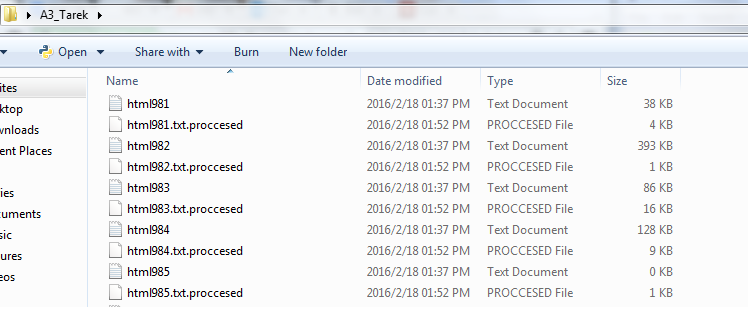
\includegraphics[scale=0.95]{fig.png}
\caption{The files I have in my directory}
\label{fig:fig.png}
\end{figure}


\newpage
\section{Problem number 2 TF-IDF}

The task in this question is to choose a word (in my case I chose `MARKET` to be the keyword), and find a list of the processed files that I have created in the first question in this assignment to be matching. The mission to count this word in all the thousand processed files was challenging. I tried to use gerp command but it printed out the whole lines in the Terminal and could not keep track of neither the number of the keyword repition nor the place.
\newpage
I found it more convenient and easier to use python to loop in each file and check if the Key word is there, also printing out the number of occurences of this word in each file and the number of files that this keyword occured in. The following is the program for such a task:

\lstinputlisting[language=Python,frame=single,caption={python code to count the keyword in the processed files},label=lst:q2code1,captionpos=b,numbers=left,
numberstyle=\tiny\color{gray},
  keywordstyle=\color{blue},
  commentstyle=\color{dkgreen},
  stringstyle=\color{mauve},showspaces=false,showstringspaces=false,basicstyle=\footnotesize]{wcount.py}
Line 4 searches for all the files that ends with `.txt.processed` in my directory, as these are the files we need to implement that program on.
Variable `fileindex` is used to keep track of the file we are iterating on,`numberoffiles` variable keeps track of the number of files that has the Keyword in and finally `wordcount` keeps track of how many times the keyword occured in every file.
\begin{figure}
\centering
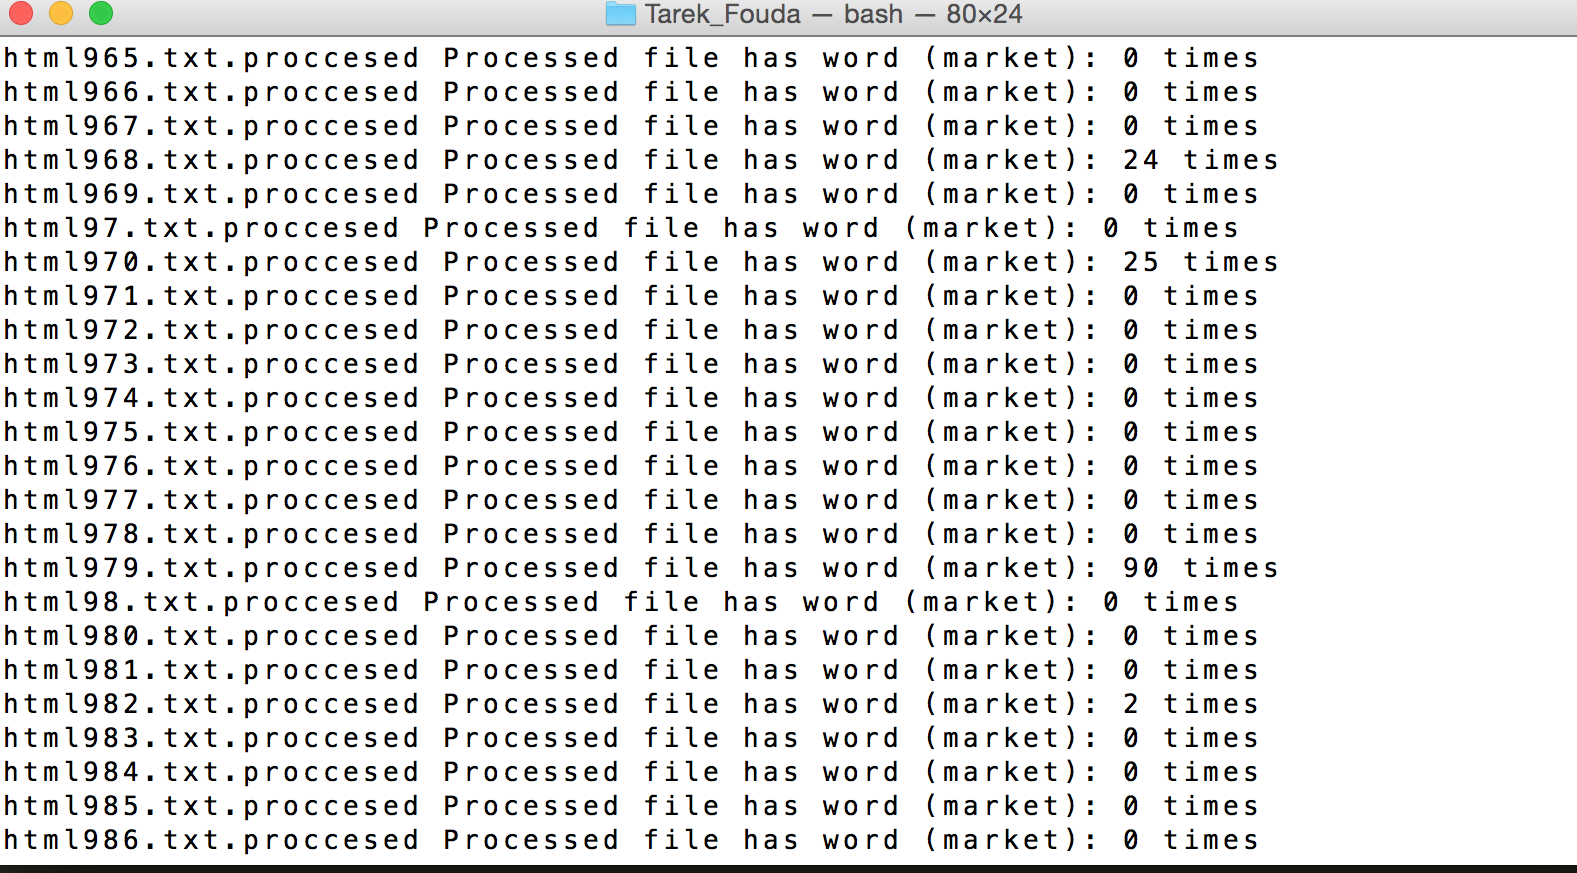
\includegraphics[scale=0.45]{1.png}
\caption{Sample for the links with the number of occurences of the keyword}
\label{fig:fig.png}
\end{figure}
\begin{figure}
\centering
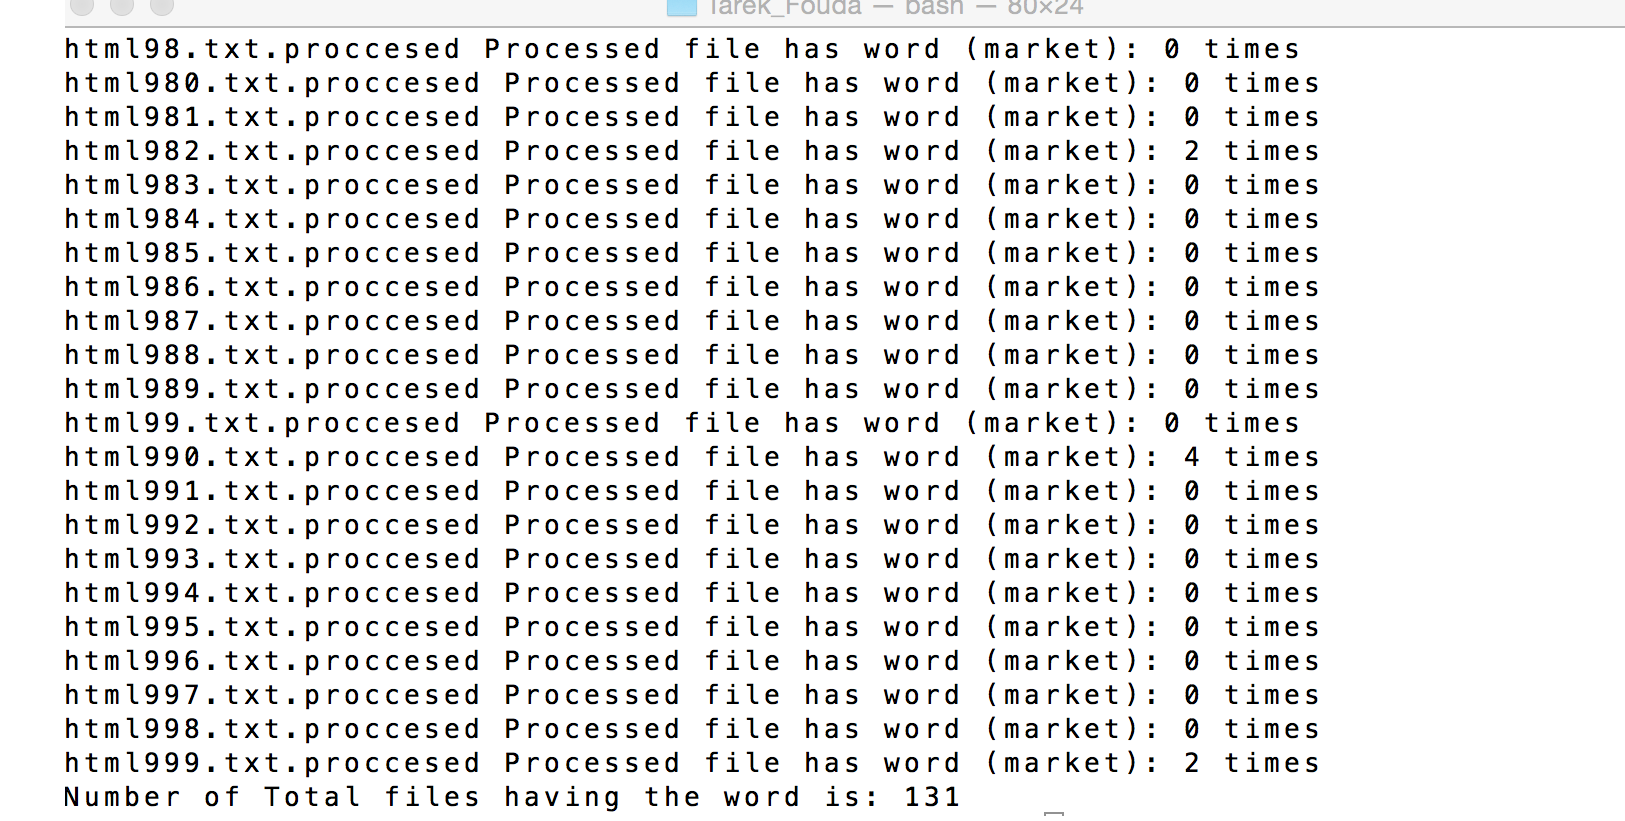
\includegraphics[scale=0.45]{2.png}
\caption{Sample for the links with the number of occurences of the keyword}
\label{fig:fig.png}
\end{figure}
The following is the table that computes TFIDF values.

 \begin{tabular}{||c c c c||} 
 \hline
TFIDF & TF & IDF & URI \\ [0.5ex] 
 \hline\hline
 0.29 & 0.07 & log2(50b/2.7B)= 4.2 & http://bit.ly/1PFA6c1 \\
\hline
 0.12 & 0.03 & log2(50b/2.7B)= 4.2 & http://onion.com/1TTlETg
 \\
 \hline
 0.0748 & 0.18 & log2(50b/2.7B)= 4.2 &http://ift.tt/1L9egku
 \\
 \hline
 0.0707 & 0.017 & log2(50b/2.7B)= 4.2 & http://buff.ly/1NRWn4i
 \\
 \hline
 0.0416 & 0.01 &log2(50b/2.7B)= 4.2 & http://compassamg.com/blog/2014/11/19
\\
\hline
 0.03328 & 0.008 & log2(50b/2.7B)= 4.2 &http://bit.ly/1o3yVMi
 \\
 \hline
 0.020 & 0.005 & log2(50b/2.7B)= 4.2 & http://bit.ly/1VUeigI
 \\
 \hline
0.012 & 0.003 & log2(50b/2.7B)= 4.2 & http://www.onlinebusinessteam.com/
 \\
 \hline
 0.010 & 0.005 & log2(50b/2.7B)= 4.2 & http://www.onlinebusinessteam.com/\\ 
 \hline
 0.002 & 0.0005 & log2(50b/2.7B)= 4.2 &http://negoogle.com//
 \\
 \hline

\end{tabular}
\newpage

TF is the keyword frequency/number of words in the document.
IDF is the log2(total docs in corpus / docs with term)
Finally the TFIDF is the multiplication of TF and IDF.
\begin{figure}
\centering
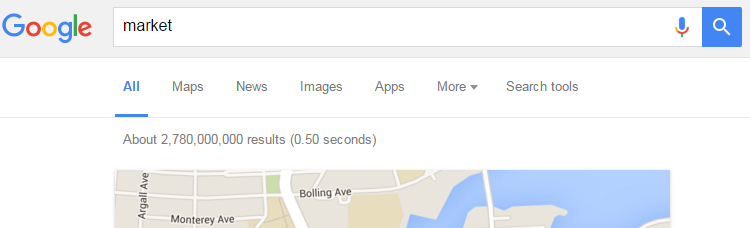
\includegraphics[scale=0.85]{3.png}
\caption{IDF}
\label{fig:fig.png}
\end{figure}
\newpage
\section{Problem number 3}

Imanually entered one of the website mentioned in the assignment to calculate the page rank for each of the 10 urls I have. 7 of the URL's gave me undefined as an answer and only 3 gave me the rank.

Also if I put the URLs as a whole it will give me undefined, so I put the root url.
Example: Instead of www.cs.odu.edu/1526/br? I put www.cs.odu.edu as it does not give me undefined.

The following is the table. 

 \begin{tabular}{||c c||} 
 \hline
Page Rank & URI  \\ [0.5ex] 
 \hline\hline
 0.7 & http://onion.com/1TTlETg  \\
\hline
 0.6& http://buff.ly/1NRWn4i 
 \\
 \hline
 0.2 & http://compassamg.com/blog/2014
 \\
 \hline
 undefined & http://negoogle.com/
 \\
 \hline
 undefined & http://mindpluckd.com/2015
\\
\hline
undefined &  http://ift.tt/1L9egku 
 \\
 \hline
 undefined & http://www.onlinebusinessteam.com/2015
 \\
 \hline
undefined & http://bit.ly/1VUeigI
 \\
 \hline
 undefined & http://bit.ly/1o3yVMi\\ 
 \hline
undefined & http://www.onlinebusinessteam.com/
 \\
 \hline

\end{tabular}
The table in figure two is basically comparing and computing the number of occurence of word market in each of the 10 links. it calculates  the frequency of this term by the rules stated in Section 2.
On the other hand the page rank table shows how popular the URL is, and does not have somthing to do with the word market.
\end{document}